\documentclass{article}

\usepackage{generalsnips}
\usepackage{calculussnips}
\usepackage[margin = 1in]{geometry}
\usepackage{pdfpages}
\usepackage[spanish]{babel}
\usepackage{amsmath}
\usepackage{amsthm}
\usepackage[utf8]{inputenc}
\usepackage{titlesec}
\usepackage{xpatch}
\usepackage{fancyhdr}
\usepackage{tikz}
\usepackage{hyperref}
\usepackage{float}
\title{Stanford Strategy and competition}
\date{2020 March 29, 11:16PM}
\author{David Gabriel Corzo Mcmath}

\begin{document}
\maketitle
%%%%%%%%%%%%%%%%%%%%%%%%%%%%%%%%%%%%%%%%%%%%%%%%%%%%%%%%%%%%%%%%%%%%%%%%%%%%%%%%%%%%%%%%%%%%%%%%%%%%%%%%%%%%%%%%%%%%%%%%%%%%%%%%%%%%%%%%%%%%%%


\section{Competition is for loosers}
\begin{itemize}
    \item When you start a company you want a monopoly.
    \item A business creates X dollars of value and captures Y\% of X. X and Y are independent variables.
    \item Air travel vs. Google. Are airlines more important than google? Intuition says yes. This explains X and Y as independent variables.
    \item Perfect competition:
        \begin{center}
            \begin{tabular}{ |l|l| }
                \hline
                    Pros & Cons \\
                \hline
                    Easy to model & Psycologically unhealthy \\ 
                    eficient in static word & irrelevant in a dynamic world \\ 
                    politically salable & preempts question of value \\ 
                \hline
            \end{tabular}
        \end{center}
    
    \item Monopoly: 
        \begin{center}
            \begin{tabular}{ |l|l| }
                \hline
                    Pros & Cons \\ 
                \hline
                    incentive to innovate & lower output, higher prices \\ 
                    Stable, long term planning & Price discrimination \\ 
                    Deeper project financing & Stifie innovation \\ 
                    Symptomatic creation & Tying \\
                \hline
            \end{tabular}
        \end{center}
    
    \item Bussiness idea: Bussinesses are either monopolies or perfectly competitive. 
    \item Diferences are quite small, anyone that has a monopoly will pretend they don't, if the market you are in is perfectly competitive you will tend to say that it is a monopoly, it's always the oposite what you say.
    \item non-monopolies: ``we're a narrow market'' A $\cap $ B $\cap$ C 
    \item monopolies: ``we're a huge market'' A $\cup $ B $\cup $  C
    \item Powerfull incentives to disort the nature of these markets.
\end{itemize}


\section{Maximizing profits under a monopoly}
\begin{itemize}
    \item Example: AIDS drugs are expensive because of monopolies.
    \item Market Power: The power to raise price above marginal cost without fear that other firms will enter the market. 
    \item In a competitive market price will fall to marginal cost, indian aids pill is 50 cents.
\end{itemize}
\subsection{Sources to market power}
Selling a uniqyue good with barriers to entry such as:
\begin{itemize}
    \item Patents.
    \item Government regulations other than patents. 
    \item Economies of scale.
    \item Exclusive access to an important input good. 
    \item Tecnological innovation. 
\end{itemize}
\subsubsection{Profit maximizing price}
When Marginal Revenue is the same as price, remember that MR is not P, therefore this is not the same idea of the perfectly competitive market. 
The monopolist faces the entire downward sloping market demand curve, as a result profits are maximized when: 
\[
  \text{ MR } < \text{ P }
\]

\begin{center}
    \begin{figure}[H]
        \centering
        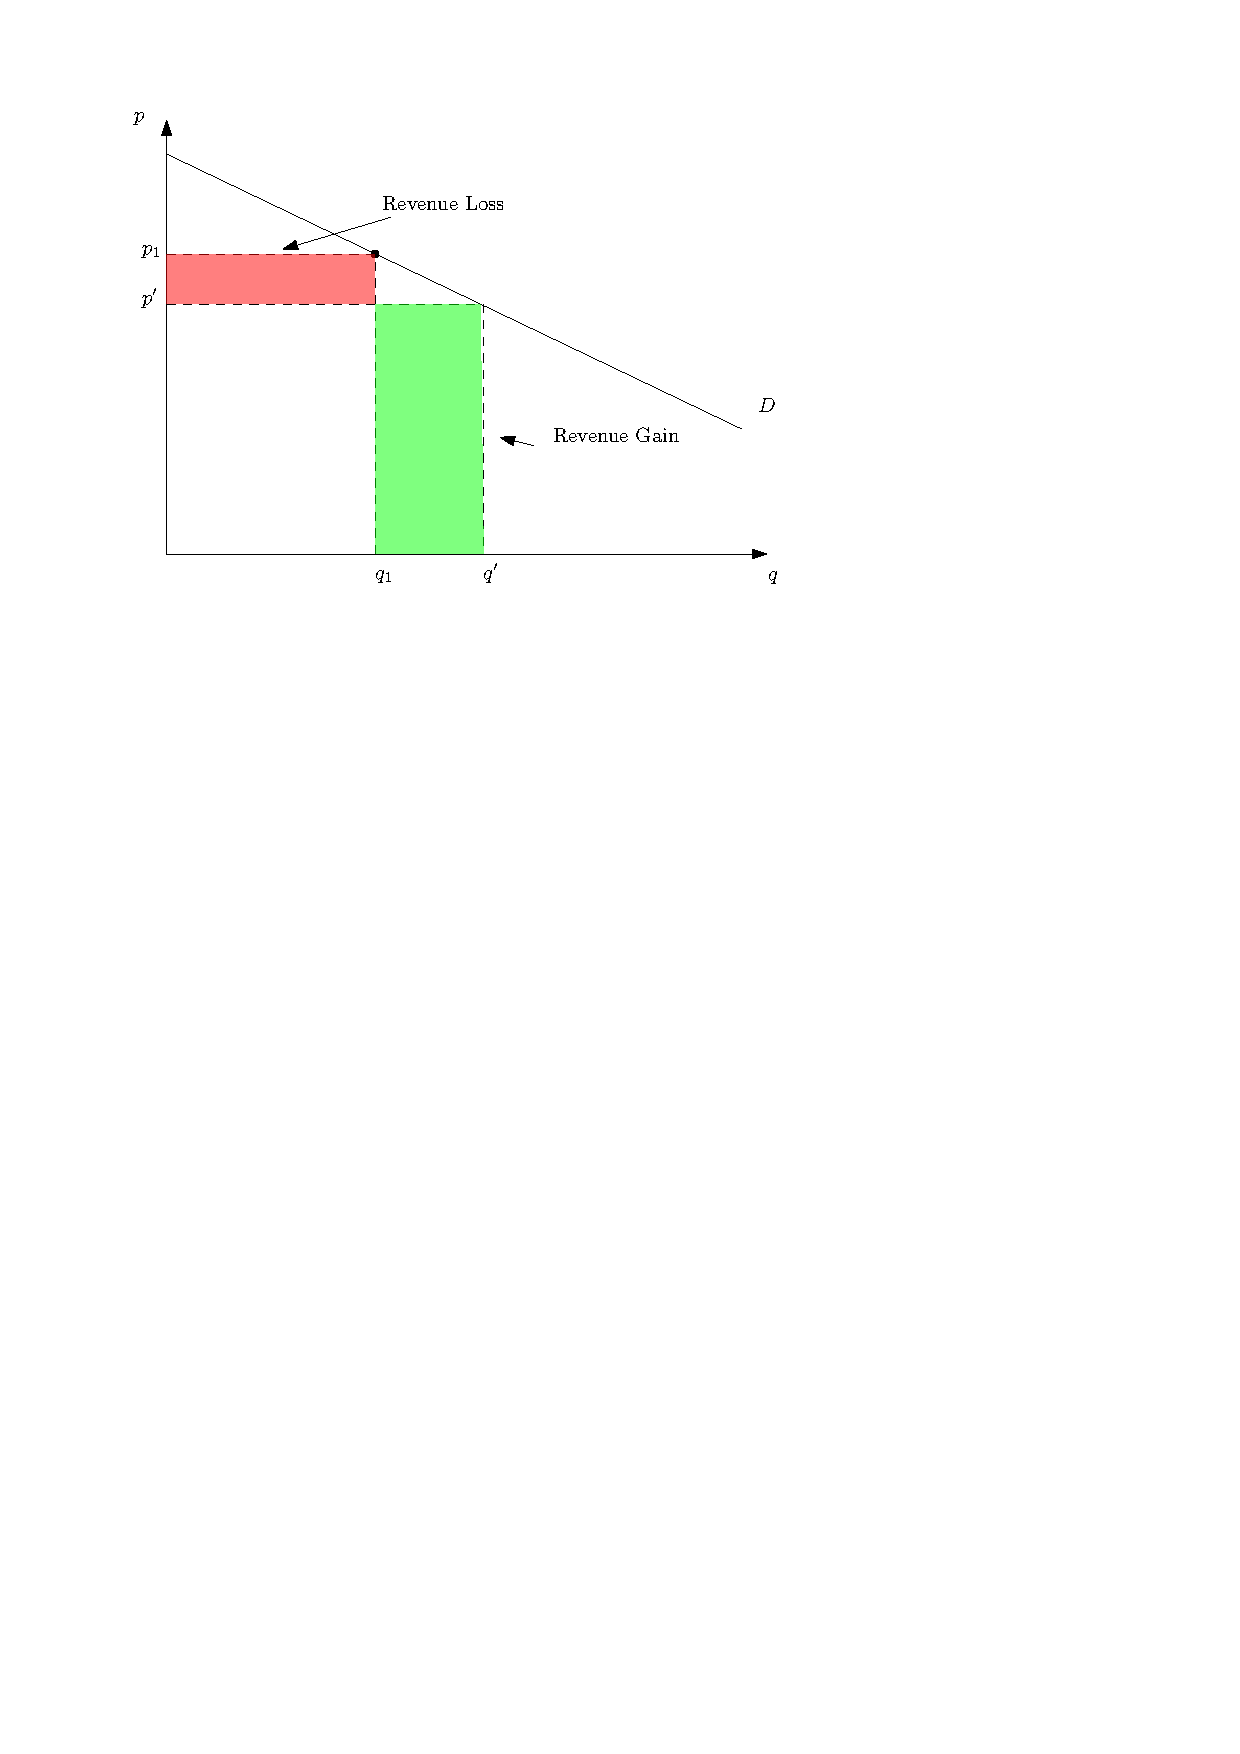
\includegraphics[]{./figs/monopoly} 
    \end{figure}    
\end{center}


%----------------------------------------------------------------------------------------
\subsection{Shortcut for calculating the monopolie's maximizing profits}
\begin{itemize}
    \item MR begins at the same point on the vertical axis. 
    \item MR has twice theslope.
\end{itemize}
\[
  MR = \frac{D}{2} 
\]
\begin{figure}[!htb]
    \centering
    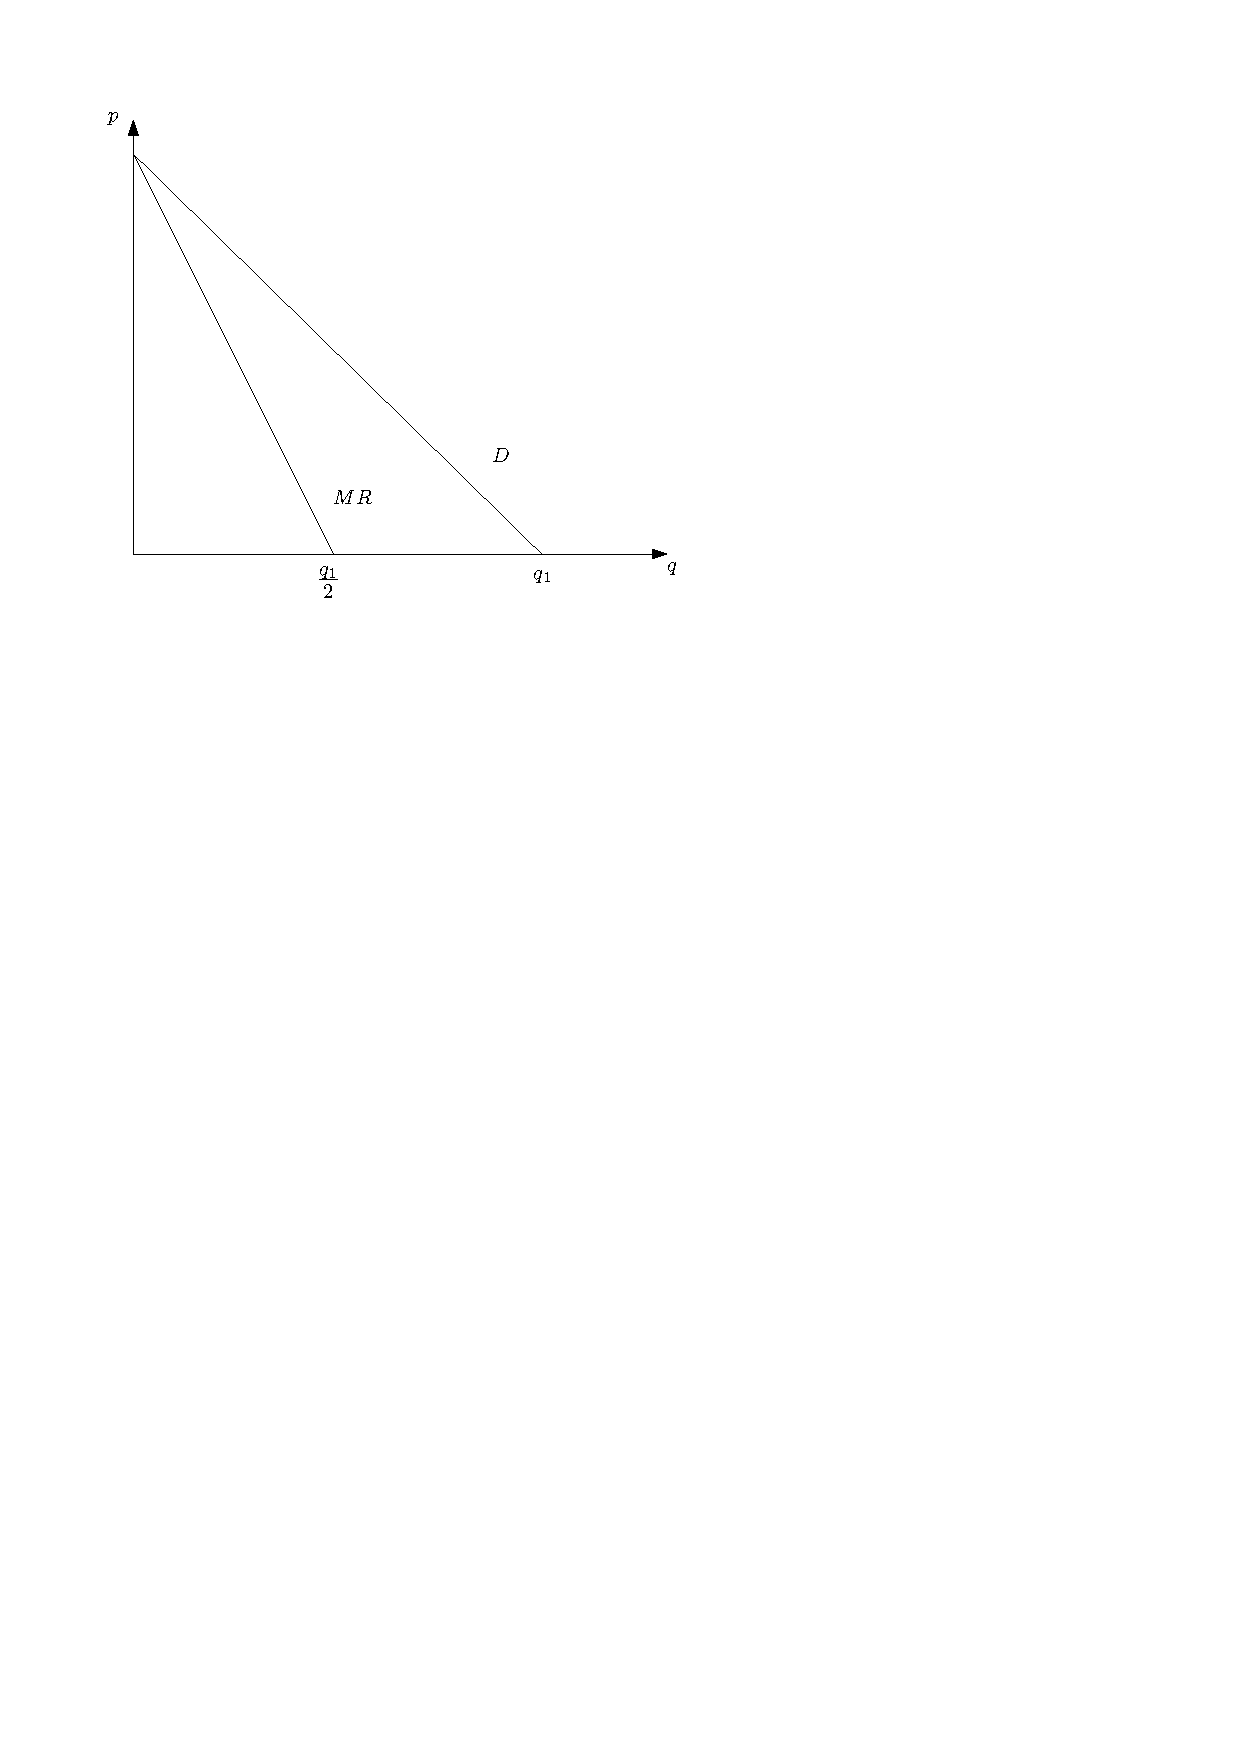
\includegraphics[]{figs/shortcut} 
\end{figure}


%----------------------------------------------------------------------------------------
\subsection{Profit}
\begin{figure}[!htb]
    \centering
    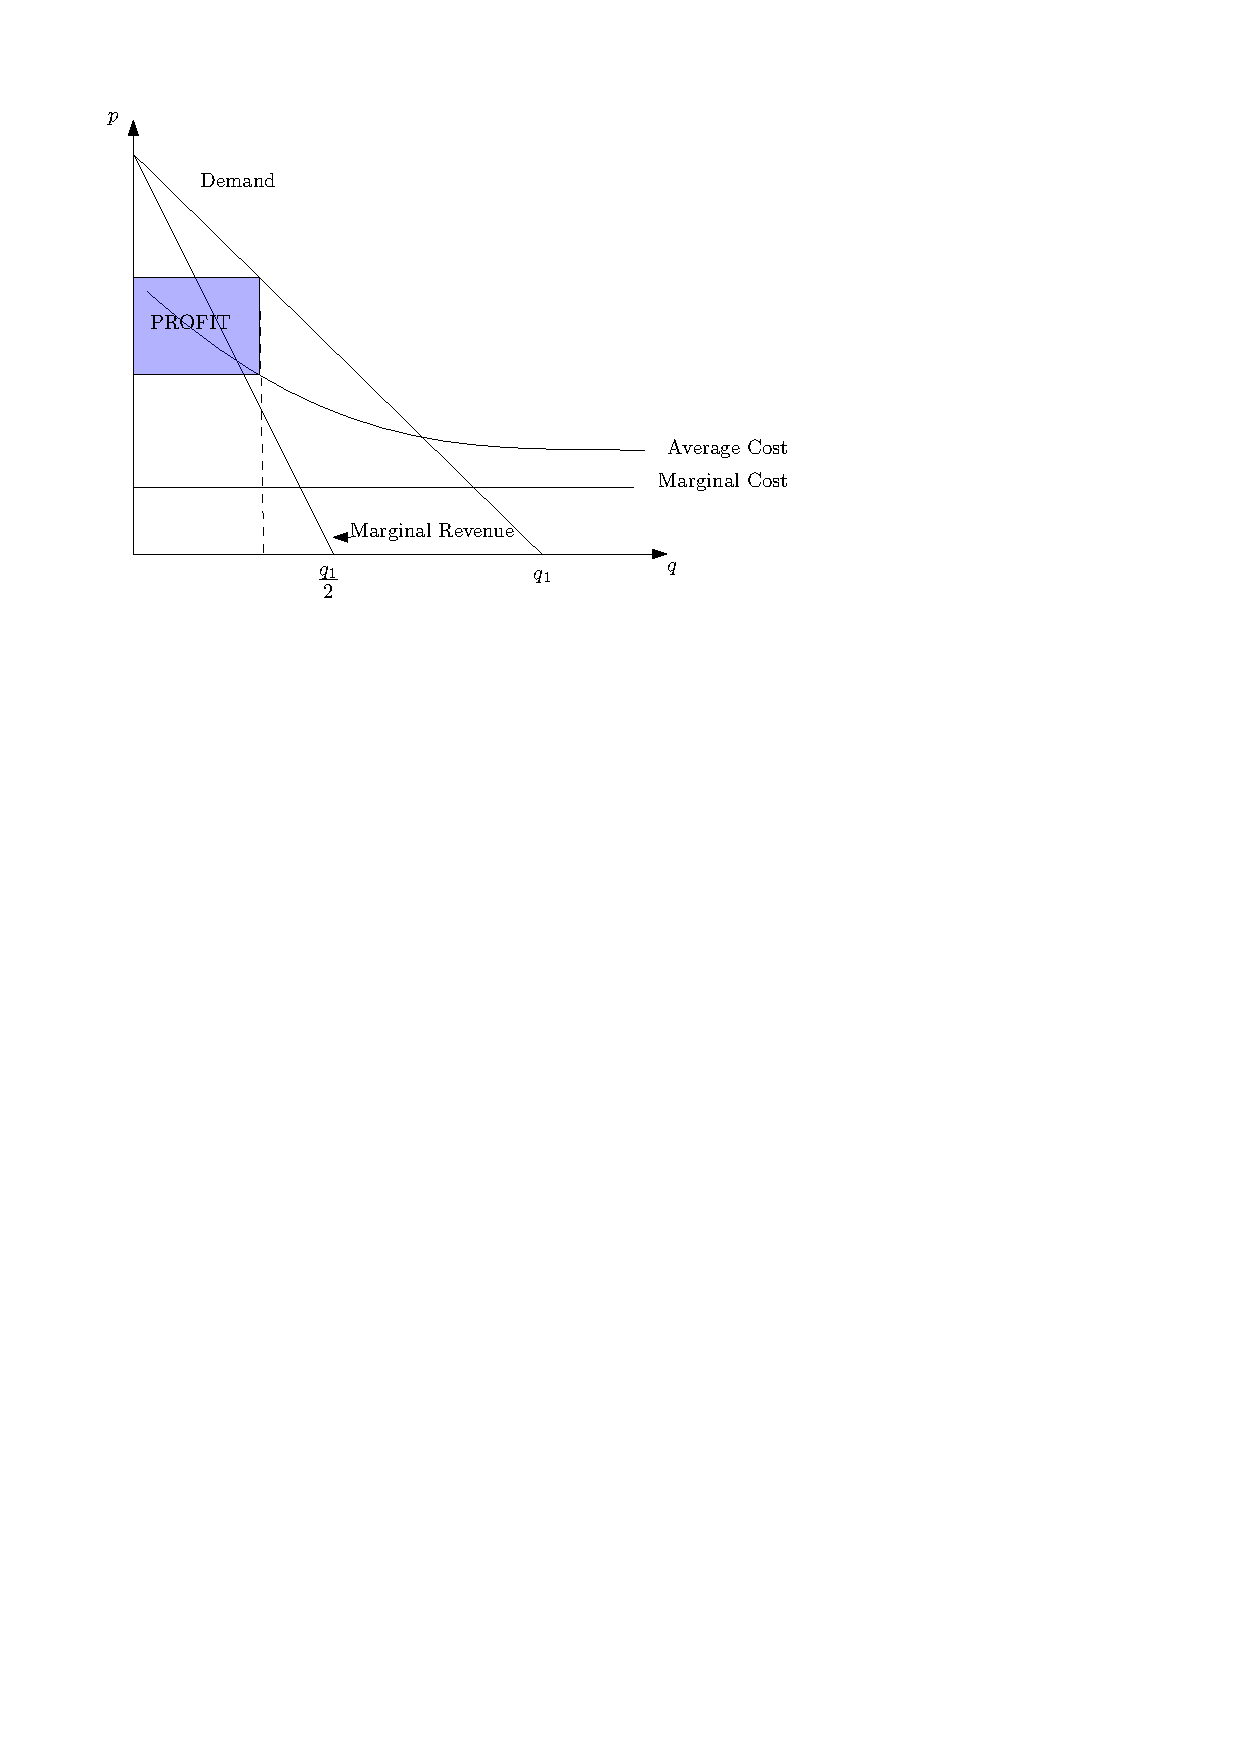
\includegraphics[]{figs/profit}
\end{figure}



%%%%%%%%%%%%%%%%%%%%%%%%%%%%%%%%%%%%%%%%%%%%%%%%%%%%%%%%%%%%%%%%%%%%%%%%%%%%%%%%%%%%%%%%%%
\section{The monopoly markup}
\begin{itemize}
    \item Two effects increse the monopoly markup:
        \begin{enumerate}
            \item The ```you can't take it with you'' effect.
            \item The ``other people's money'' effect.
        \end{enumerate}
    
    \item The less sensative quantity demanded is to price the higher the markup, i.e. the more elastic demand the higher the monopoly markup. 
\end{itemize}


%----------------------------------------------------------------------------------------
\subsection{Markup}
\begin{itemize}
    \item The more inelastic demand, the bigger the markup. 
\end{itemize}
\begin{figure}[!htb]
    \centering
    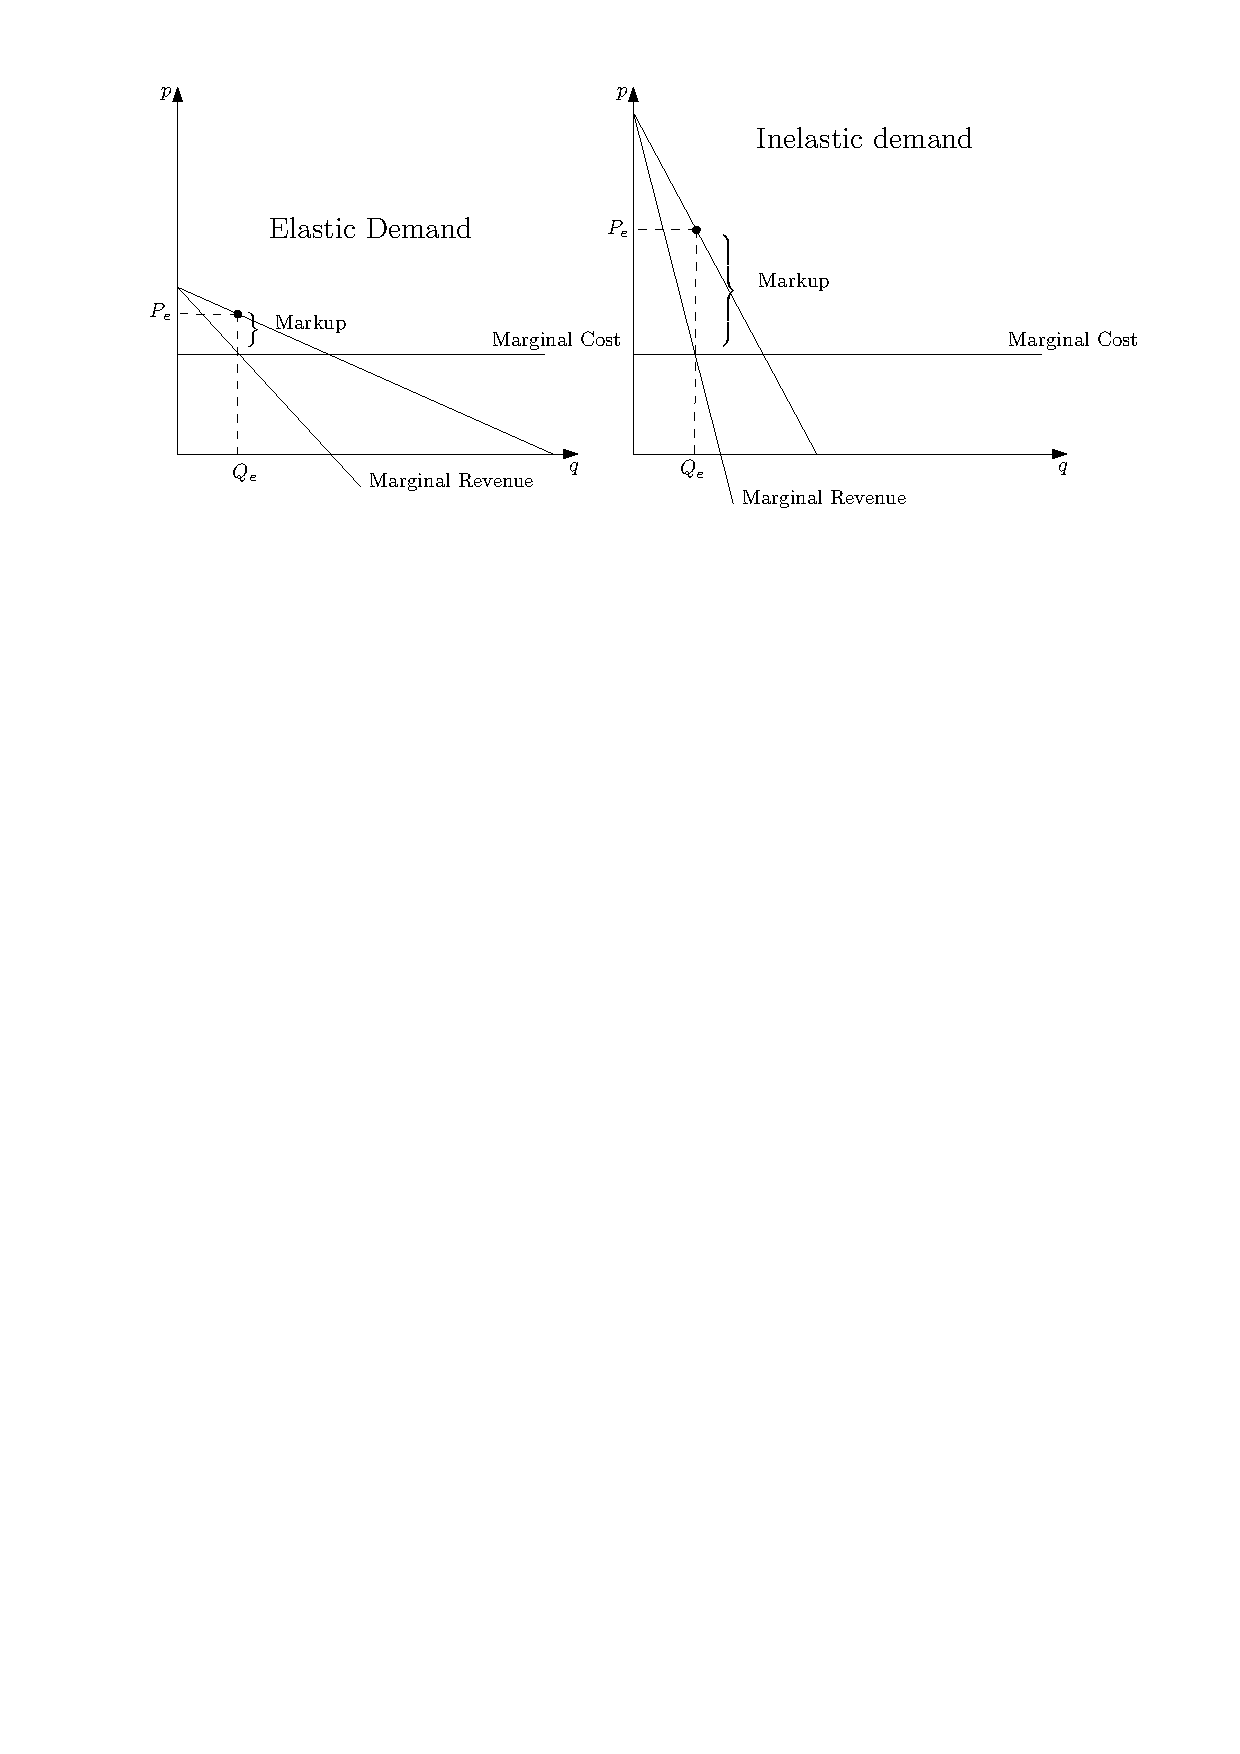
\includegraphics[]{figs/markup} 
\end{figure}



%%%%%%%%%%%%%%%%%%%%%%%%%%%%%%%%%%%%%%%%%%%%%%%%%%%%%%%%%%%%%%%%%%%%%%%%%%%%%%%%%%%%%%%%%%%%%%%%%%%%%%%%%%%%%%%%%%%%%%%%%%%%%%%%%%%%%%%%%%%%%%
\end{document}

